% -*- latex -*-
%%%%%%%%%%%%%%%%%%%%%%%%%%%%%%%%%%%%%%%%%%%%%%%%%%%%%%%%%%%%%%%%
%%%%%%%%%%%%%%%%%%%%%%%%%%%%%%%%%%%%%%%%%%%%%%%%%%%%%%%%%%%%%%%%
%%%%
%%%% This text file is part of the source of 
%%%% `Parallel Programming in MPI and OpenMP'
%%%% by Victor Eijkhout, copyright 2012-9
%%%%
%%%% mpi-morecollective.tex : obscure stuff
%%%%
%%%%%%%%%%%%%%%%%%%%%%%%%%%%%%%%%%%%%%%%%%%%%%%%%%%%%%%%%%%%%%%%
%%%%%%%%%%%%%%%%%%%%%%%%%%%%%%%%%%%%%%%%%%%%%%%%%%%%%%%%%%%%%%%%

\Level 0 {MPI Operators}
\index{operator|(}

MPI \emph{operators} are used in reduction operators. Most common
operators, such as sum or maximum, have been built into the MPI
library, but it is possible to define new operators.

\Level 1 {Pre-defined operators}
\label{sec:operator-list}

The following is the list of \emph{pre-defined operators}\index{operator!predefined}
\indexmpidef{MPI_OP} values.

{\catcode`\_=12 %pyskip
  \begin{tabular}{|lll|}
    \hline
  MPI type&meaning&applies to\\ \hline
  \indexmpidef{MPI_MAX}&maximum&integer, floating point\\
  \indexmpidef{MPI_MIN}&minimum&\\
  \indexmpidef{MPI_SUM}&sum&integer, floating point, complex,
  multilanguage types\\
  \indexmpidef{MPI_PROD}&product&\\
  \indexmpidef{MPI_LAND}&logical and&C integer, logical\\
  \indexmpidef{MPI_LOR}&logical or&\\
  \indexmpidef{MPI_LXOR}&logical xor&\\
  \indexmpidef{MPI_BAND}&bitwise and&integer, byte, multilanguage types\\
  \indexmpidef{MPI_BOR}&bitwise or&\\
  \indexmpidef{MPI_BXOR}&bitwise xor&\\
  \indexmpidef{MPI_MAXLOC}&max value and
  location&\indexmpishow{MPI_DOUBLE_INT} and such\\
  \indexmpidef{MPI_MINLOC}&min value and location&\\
  \hline
\end{tabular}
} %pyskip

The \indexmpishow{MPI_MAXLOC} operation yields both the maximum and
the rank on which it occurs. However, to use it the input should be an
array of \n{real/int} structs, where the \n{int} is the rank of the number.

\Level 1 {User-defined operators}
\label{sec:mpi-op-create}

In addition to predefined operators, MPI has the possibility of
\emph{user-defined operators}\index{operator!user-defined}
to use in a reduction or scan operation.

\mpiRoutineRef{MPI_Op_create}

The function needs to have the following prototype:

\begin{verbatim}
typedef void MPI_User_function
    ( void *invec, void *inoutvec, int *len, 
      MPI_Datatype *datatype); 

FUNCTION USER_FUNCTION( INVEC(*), INOUTVEC(*), LEN, TYPE) 
<type> INVEC(LEN), INOUTVEC(LEN) 
INTEGER LEN, TYPE 
\end{verbatim}

The function has an array length argument~\n{len}, to allow for
pointwise reduction on a whole array at once. The \n{inoutvec} array
contains partially reduced results, and is typically overwritten by
the function.

There are some restrictions on the user function:
\begin{itemize}
\item It may not call MPI functions, except for
  \indexmpishow{MPI_Abort}.
\item It must be associative; it can be optionally commutative, which
  fact is passed to the \indexmpishow{MPI_Op_create} call.
\end{itemize}

For example, here is an operator for finding the smallest non-zero
number in an array of nonnegative integers:
%
\cverbatimsnippet{mpirwz}

\begin{exercise}
  \label{ex:one-norm-op}
  Write the reduction function to implement the
  \emph{one-norm}\index{norm!one} of a vector:
  \[ \|x\|_1 \equiv \sum_i |x_i|. \]
\end{exercise}

You can query the commutativity of an operator:
%
\mpiRoutineRef{MPI_Op_commutative}

A created \indexmpishow{MPI_Op} can be freed again:
%
\begin{lstlisting}
int MPI_Op_free(MPI_Op *op)
\end{lstlisting}
%
This sets the operator to \indexmpishow{MPI_OP_NULL}.

\Level 1 {Local reduction}

The application of an \indexmpishow{MPI_Op} can be performed with the routine
\indexmpishow{MPI_Reduce_local}. Using this routine and some
send/receive scheme you can build your own global reductions. Note
that this routine does not take a communicator because it is purely local.

\mpiRoutineRef{MPI_Reduce_local}

\index{operator|)}

\Level 0 {Non-blocking collectives}
\label{sec:mpi3collect}

Above you have seen how the `Isend' and `Irecv' routines can overlap communication
with computation. This is not possible with the collectives you have seen so far:
they act like blocking sends or receives.
However, there are also \indextermsub{non-blocking}{collectives}.
These have roughly the same calling sequence as their blocking counterparts,
except that they output an \indexmpishow{MPI_Request}. You
can then use an \indexmpishow{MPI_Wait} call to make sure the collective
has completed.

Such operations can be used to increase efficiency.
For instance, computing
\[ y \leftarrow Ax + (x^tx)y \]
involves a matrix-vector product, which is dominated by computation
in the \indextermsub{sparse}{matrix} case, and an inner product which is 
typically dominated by the communication cost. You would code this as
\begin{lstlisting}
MPI_Iallreduce( .... x ..., &request);
// compute the matrix vector product
MPI_Wait(request);
// do the addition
\end{lstlisting}

This can also be used for 3D FFT operations~\cite{Hoefler:case-for-nbc}.
Occasionally, a non-blocking collective can be used for non-obvious purposes,
such as the \indexmpishow{MPI_Ibarrier} in~\cite{Hoefler:2010:SCP}.

The same calling sequence as the blocking counterpart, except for the addition
of an \indexmpishow{MPI_Request} parameter. For instance 
\indexmpishow{MPI_Ibcast}:
\begin{lstlisting}
int MPI_Ibcast(
  void *buffer, int count, MPI_Datatype datatype,
  int root, MPI_Comm comm, 
  MPI_Request *request)
\end{lstlisting}

Non-blocking collectives offer a number of performance advantages:
\begin{itemize}
\item Do two reductions (on the same communicator) with different
  operators simultaneously;
\item do collectives on overlapping communicators simultaneously;
\item overlap a non-blocking collective with a blocking one. (However,
  note that blocking and non-blocking don't match: either all process 
  call the non-blocking or all call the blocking one.)
\end{itemize}

\begin{exercise}
  \label{ex:procgridnonblock}
  Revisit exercise~\ref{ex:rowcolcomm}. Let only the first row and
  first column have certain data, which they broadcast through columns
  and rows respectively. Each process is now involved in two
  simultaneous collectives. Implement this with non-blocking
  broadcasts, and time the difference between a blocking and a
  non-blocking solution.
\end{exercise}

\mpiRoutineRef{MPI_Ibcast}

\mpiRoutineRef{MPI_Iallreduce}

\mpiRoutineRef{MPI_Iallgather}

\Level 1 {Non-blocking barrier}
\label{sec:ibarrier}

Probably the most surprising non-blocking collective is the
\indextermsub{non-blocking}{barrier}
\indexmpishow{MPI_Ibarrier}. The way to understand this is to think of
a barrier not in terms of temporal synchronization, but state
agreement: reaching a barrier is a sign that a process has attained a
certain state, and leaving a barrier means that all processes are in
the same state. The ordinary barrier is then a blocking wait for
agreement, while with a non-blocking barrier:
\begin{itemize}
\item Posting the barrier means that a process has reached a certain
  state; and
\item the request being fullfilled means that all processes have
  reached the barrier.
\end{itemize}

\mpiRoutineRef{MPI_Ibarrier}

We can use a non-blocking barrier to good effect, utilizing the idle
time that would result from a blocking barrier. In the following code
fragment processes test for completion of the barrier, and failing to
detect such completion, perform some local work.

\cverbatimsnippet{ibarrierpoll}

\Level 0 {Performance of collectives}

It is easy to visualize a broadcast as in figure~\ref{fig:bcast-simple}:
see figure~\ref{fig:bcast-simple}.
\begin{figure}[ht]
  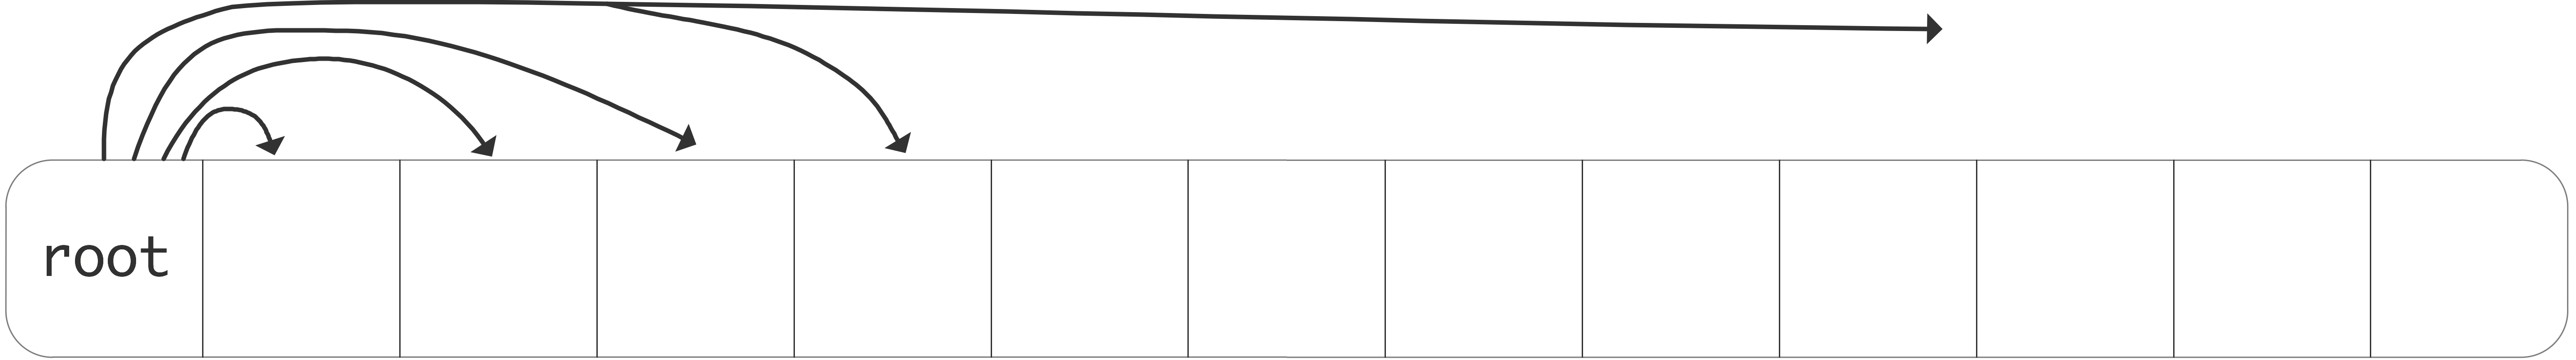
\includegraphics[scale=.08]{graphics/bcast-simple}
  \caption{A simple broadcast}
  \label{fig:bcast-simple}
\end{figure}
the root sends all of its data directly to every other process.
While this describes the semantics of the operation, in practice
the implementation works quite differently.

The time that a message takes can simply be modeled as
\[ \alpha +\beta n, \]
where $\alpha$~is the \indexterm{latency}, a~one time
delay from establishing the communication between two processes,
and $\beta$~is the time-per-byte, or the inverse of the \indexterm{bandwidth},
and $n$~the number of bytes sent.

Under the assumption that
a processor can only send one message at a time,
the broadcast in
figure~\ref{fig:bcast-simple} would take a time proportional to the
number of processors.

\begin{exercise}
  \label{ex:latencylinear}
  What is the total time required for a broadcast involving $p$
  processes?
  Give $\alpha$ and $\beta$ terms separately.
\end{exercise}

One way to ameliorate that is to structure the
broadcast in a tree-like fashion.
\begin{figure}[ht]
  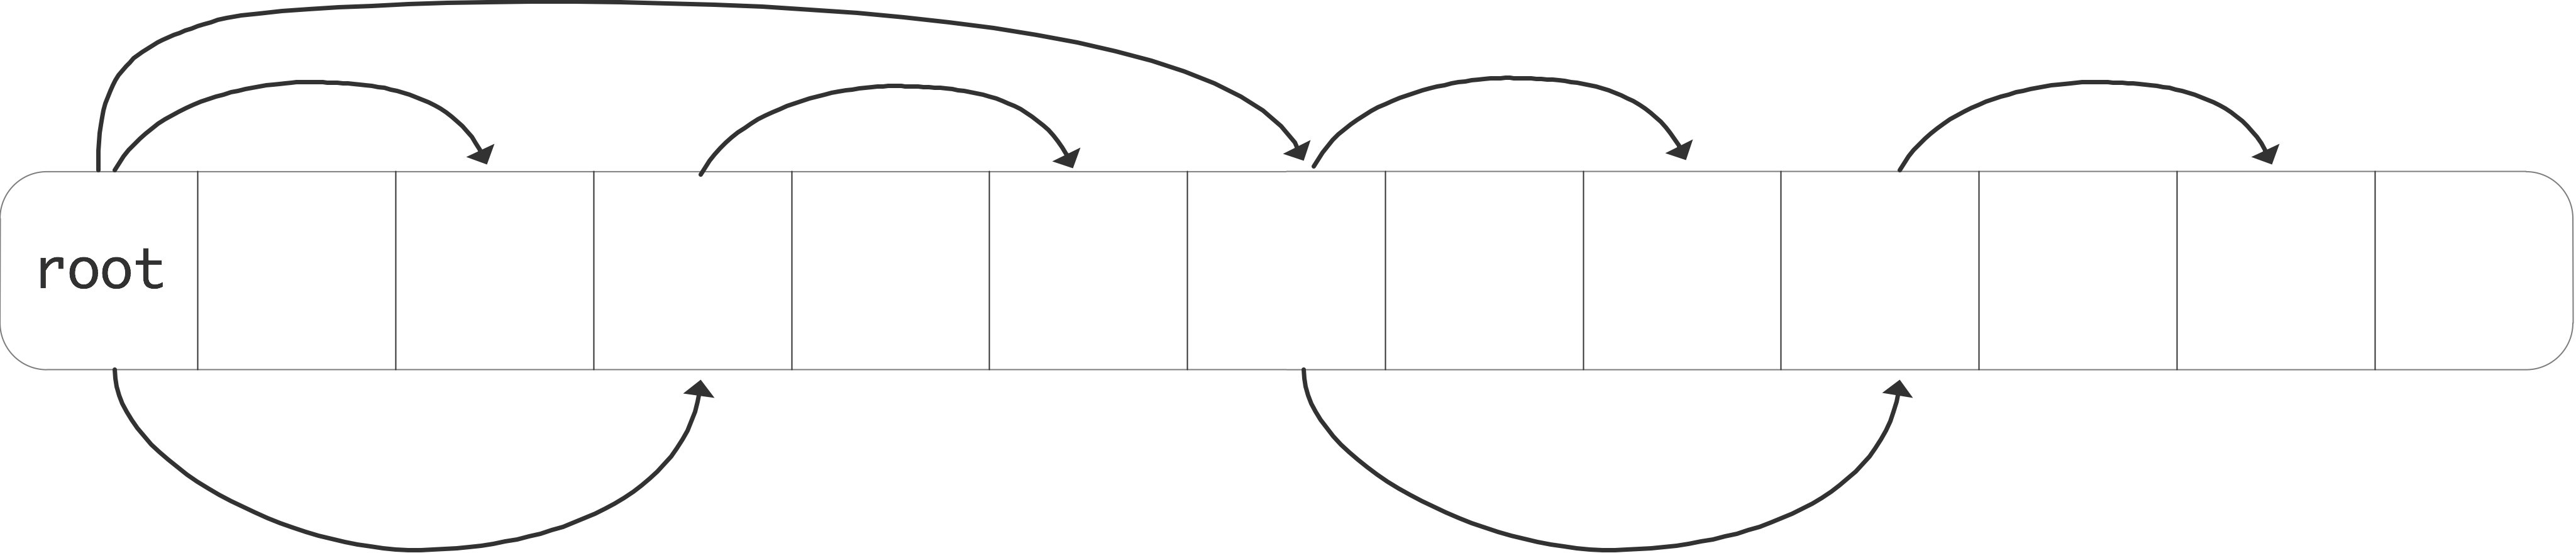
\includegraphics[scale=.1]{graphics/bcast-tree}
  \caption{A tree-based broadcast}
  \label{fig:bcast-tree}
\end{figure}
This is depicted in figure~\ref{fig:bcast-tree}.

\begin{exercise}
  \label{ex:latencylog}
  How does the
  communication time now depend on the number of processors, again
  $\alpha$ and $\beta$ terms separately.

  What would be a lower bound on the $\alpha,\beta$ terms?
\end{exercise}

The theory
of the complexity of collectives is described in more detail in
\HPSCref{sec:collective}; see also~\cite{Chan2007Collective}.

\Level 0 {Collectives and synchronization}

Collectives, other than a barrier, have a synchronizing effect between processors.
For instance, in
\begin{lstlisting}
MPI_Bcast( ....data... root);
MPI_Send(....);
\end{lstlisting}
the send operations on all processors will occur after the root executes
the broadcast. 
\begin{figure}[ht]
  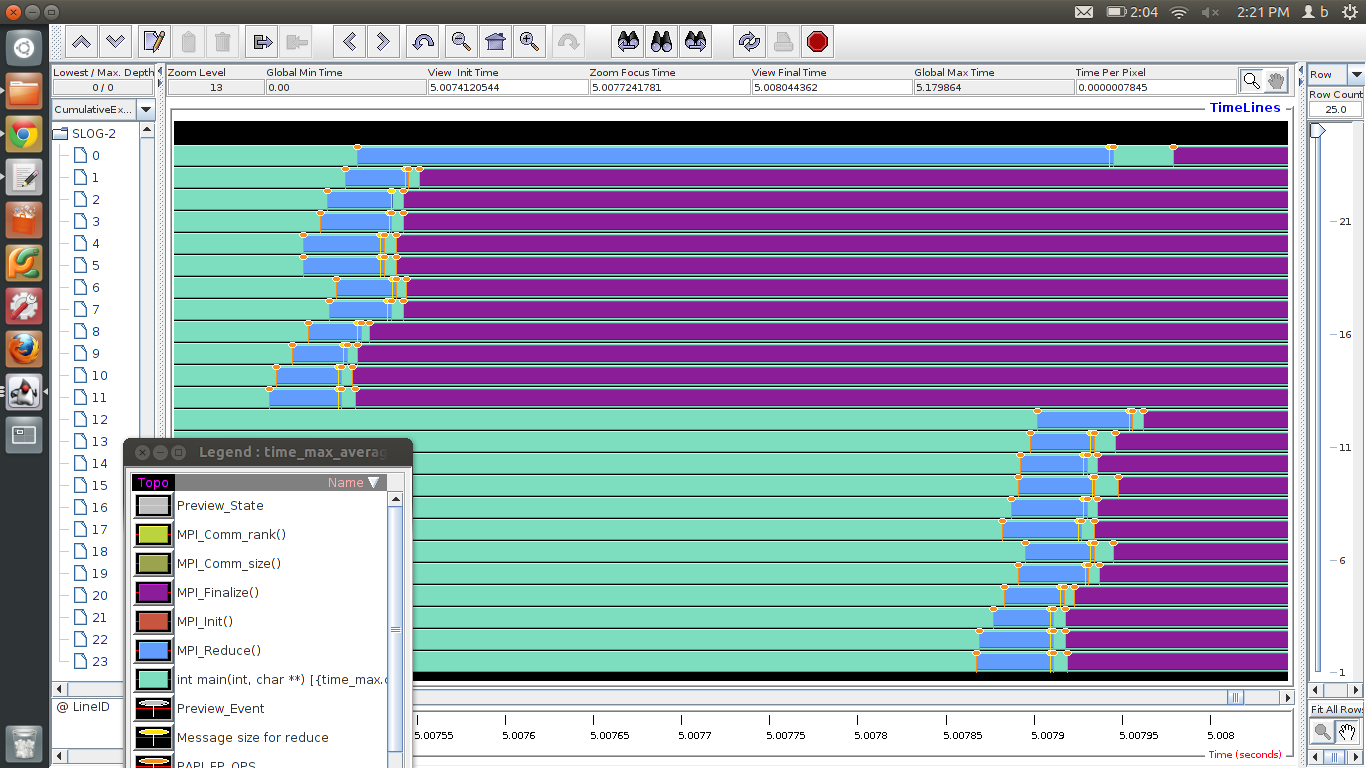
\includegraphics[scale=.35]{graphics/reduce-two-node}
  \caption{Trace of a reduction operation between two dual-socket 12-core nodes}
  \label{fig:trace-reduce}
\end{figure}
Conversely, in a reduce operation the root may have to wait for 
other processors. This is illustrated in figure~\ref{fig:trace-reduce}, which 
gives a TAU trace of
a reduction operation on two nodes, with two six-core sockets (processors) each.
We see that\footnote
{This uses mvapich version 1.6; in version 1.9 the implementation of an on-node reduction
has changed to simulate shared memory.}:
\begin{itemize}
\item In each socket, the reduction is a linear accumulation;
\item on each node, cores zero and six then combine their result;
\item after which the final accumulation is done through the network.
\end{itemize}
We also see that the two nodes are not perfectly in sync, which is normal for MPI
applications. As a result, core~0 on the first node will sit idle until it receives the partial
result from core~12, which is on the second node.

\begin{figure}[p]
  \footnotesize
  \leftskip=\unitindent
  \rightskip=\unitindent
Code:
{\tiny
\begin{lstlisting}
switch(rank) { 
    case 0: 
        MPI_Bcast(buf1, count, type, 0, comm); 
        MPI_Send(buf2, count, type, 1, tag, comm); 
        break; 
    case 1: 
        MPI_Recv(buf2, count, type, MPI_ANY_SOURCE, tag, comm, status); 
        MPI_Bcast(buf1, count, type, 0, comm); 
        MPI_Recv(buf2, count, type, MPI_ANY_SOURCE, tag, comm, status); 
        break; 
    case 2: 
        MPI_Send(buf2, count, type, 1, tag, comm); 
        MPI_Bcast(buf1, count, type, 0, comm); 
        break; 
}
\end{lstlisting}
}
The most logical execution is:\par\medskip

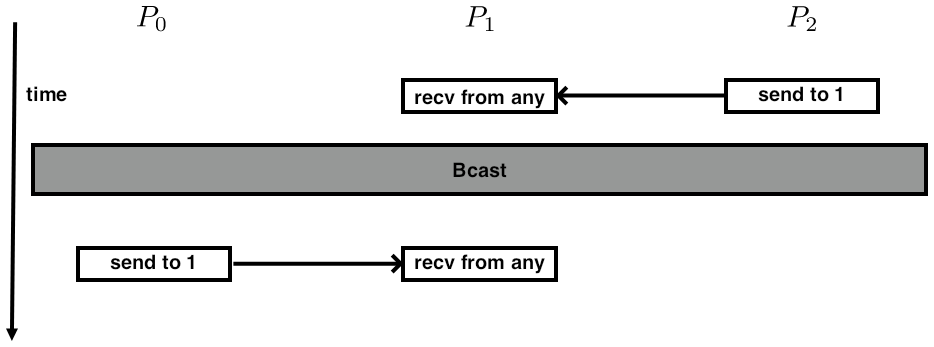
\includegraphics[scale=.35]{backintime1}

However, this ordering is allowed too:\par\medskip

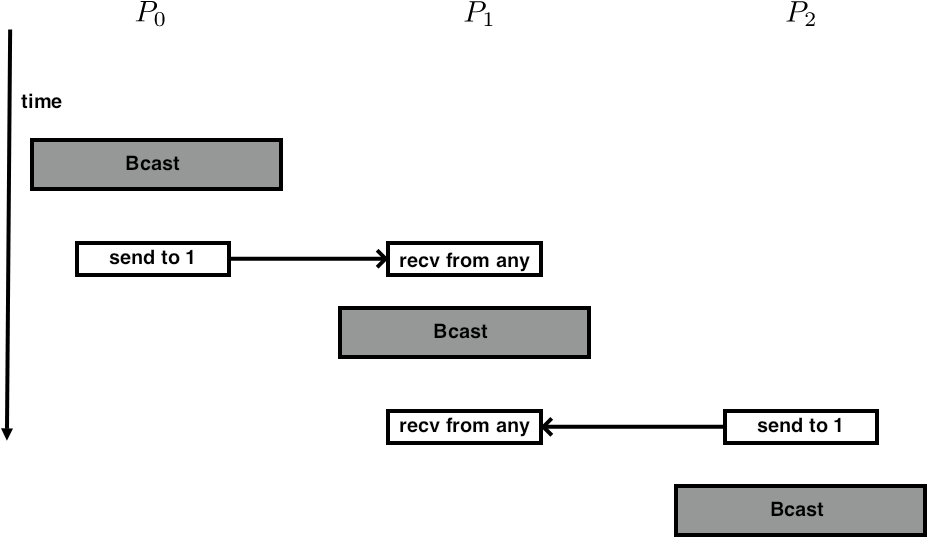
\includegraphics[scale=.35]{backintime2}

Which looks from a distance like:\par\medskip

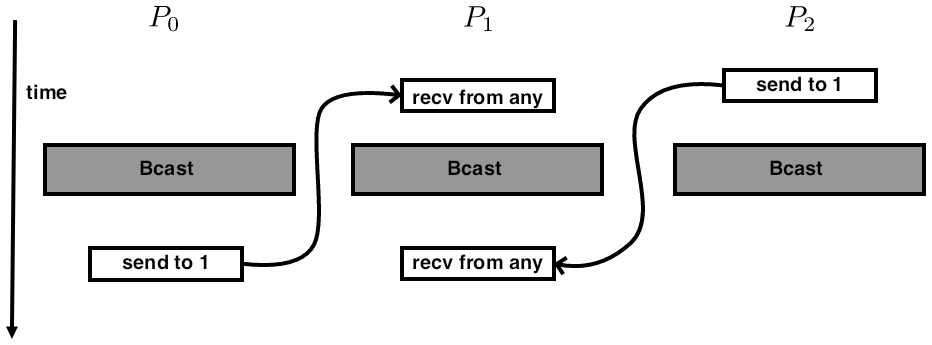
\includegraphics[scale=.35]{backintime3}

In other words, one of the messages seems to go `back in time'.

  \caption{Possible temporal orderings of send and collective calls}
  \label{fig:backintime}
\end{figure}

While collectives synchronize in a loose sense, it is not possible to
make any statements about events before and after the collectives
between processors:
\begin{lstlisting}
...event 1...
MPI_Bcast(....);
...event 2....
\end{lstlisting}
Consider a specific scenario:
\begin{lstlisting}
switch(rank) { 
    case 0: 
        MPI_Bcast(buf1, count, type, 0, comm); 
        MPI_Send(buf2, count, type, 1, tag, comm); 
        break; 
    case 1: 
        MPI_Recv(buf2, count, type, MPI_ANY_SOURCE, tag, comm, status); 
        MPI_Bcast(buf1, count, type, 0, comm); 
        MPI_Recv(buf2, count, type, MPI_ANY_SOURCE, tag, comm, status); 
        break; 
    case 2: 
        MPI_Send(buf2, count, type, 1, tag, comm); 
        MPI_Bcast(buf1, count, type, 0, comm); 
        break; 
}
\end{lstlisting}
Note the \indexmpishow{MPI_ANY_SOURCE} parameter in the receive calls on processor~1.
One obvious execution of this would be:
\begin{enumerate}
\item The send from~2 is caught by processor~1;
\item Everyone executes the broadcast;
\item The send from~0 is caught by processor~1.
\end{enumerate}
However, it is equally possible to have this execution:
\begin{enumerate}
\item Processor~0 starts its broadcast, then executes the send;
\item Processor~1's receive catches the data from~0, then it executes
  its part of the broadcast;
\item Processor~1 catches the data sent by~2, and finally processor~2
  does its part of the broadcast.
\end{enumerate}

This is illustrated in figure~\ref{fig:backintime}.
